\documentclass[dvipsnames]{beamer}\usepackage[]{graphicx}\usepackage[]{color}
%% maxwidth is the original width if it is less than linewidth
%% otherwise use linewidth (to make sure the graphics do not exceed the margin)
\makeatletter
\def\maxwidth{ %
  \ifdim\Gin@nat@width>\linewidth
    \linewidth
  \else
    \Gin@nat@width
  \fi
}
\makeatother

\definecolor{fgcolor}{rgb}{0.345, 0.345, 0.345}
\newcommand{\hlnum}[1]{\textcolor[rgb]{0.686,0.059,0.569}{#1}}%
\newcommand{\hlstr}[1]{\textcolor[rgb]{0.192,0.494,0.8}{#1}}%
\newcommand{\hlcom}[1]{\textcolor[rgb]{0.678,0.584,0.686}{\textit{#1}}}%
\newcommand{\hlopt}[1]{\textcolor[rgb]{0,0,0}{#1}}%
\newcommand{\hlstd}[1]{\textcolor[rgb]{0.345,0.345,0.345}{#1}}%
\newcommand{\hlkwa}[1]{\textcolor[rgb]{0.161,0.373,0.58}{\textbf{#1}}}%
\newcommand{\hlkwb}[1]{\textcolor[rgb]{0.69,0.353,0.396}{#1}}%
\newcommand{\hlkwc}[1]{\textcolor[rgb]{0.333,0.667,0.333}{#1}}%
\newcommand{\hlkwd}[1]{\textcolor[rgb]{0.737,0.353,0.396}{\textbf{#1}}}%

\usepackage{framed}
\makeatletter
\newenvironment{kframe}{%
 \def\at@end@of@kframe{}%
 \ifinner\ifhmode%
  \def\at@end@of@kframe{\end{minipage}}%
  \begin{minipage}{\columnwidth}%
 \fi\fi%
 \def\FrameCommand##1{\hskip\@totalleftmargin \hskip-\fboxsep
 \colorbox{shadecolor}{##1}\hskip-\fboxsep
     % There is no \\@totalrightmargin, so:
     \hskip-\linewidth \hskip-\@totalleftmargin \hskip\columnwidth}%
 \MakeFramed {\advance\hsize-\width
   \@totalleftmargin\z@ \linewidth\hsize
   \@setminipage}}%
 {\par\unskip\endMakeFramed%
 \at@end@of@kframe}
\makeatother

\definecolor{shadecolor}{rgb}{.97, .97, .97}
\definecolor{messagecolor}{rgb}{0, 0, 0}
\definecolor{warningcolor}{rgb}{1, 0, 1}
\definecolor{errorcolor}{rgb}{1, 0, 0}
\newenvironment{knitrout}{}{} % an empty environment to be redefined in TeX

\usepackage{alltt}
\usepackage{color} % for colors
\usepackage{graphicx}
\usepackage{hyperref}
\usepackage{svg}
\usepackage{amsmath}
\hypersetup{
    bookmarks=true,         % show bookmarks bar?
    unicode=false,          % non-Latin characters in Acrobat?s bookmarks
    pdftoolbar=true,        % show Acrobat?s toolbar?
    pdfmenubar=true,        % show Acrobat?s menu?
    pdffitwindow=false,     % window fit to page when opened
    pdfstartview={FitH},    % fits the width of the page to the window
    pdftitle={My title},    % title
    pdfauthor={Author},     % author
    pdfsubject={Subject},   % subject of the document
    pdfcreator={Creator},   % creator of the document
    pdfproducer={Producer}, % producer of the document
    pdfkeywords={keyword1} {key2} {key3}, % list of keywords
    pdfnewwindow=true,      % links in new PDF window
    colorlinks=true,       % false: boxed links; true: colored links
    linkcolor=red,          % color of internal links (change box color with linkbordercolor)
    citecolor=green,        % color of links to bibliography
    filecolor=magenta,      % color of file links
    urlcolor=blue         % color of external links
}
% \usepackage{beamerthemesplit} // Activate for custom appearance

\usecolortheme{beaver}
\title{E-411-PRMA}
\subtitle{Lecture 2}
\author{Christopher David Desjardins}
\date{20 August 2015}
\IfFileExists{upquote.sty}{\usepackage{upquote}}{}
\begin{document}







\frame{\titlepage}

%\section[Outline]{}
%\frame{\tableofcontents}

\begin{frame}
  \frametitle{SAT}
  
  The SAT is an aptitude test that high school students take. It is one of the criteria that is used in a college's decision to admit a student. It is composed of a math and a verbal section. Each has a mean of 500 and a standard devation of 110 and is normally distributed. 
  \begin{itemize}
  \item<1-> What are the scores on the test that corresponds to 3, 2, 1, 0, -1, -2, -3 standard deviations?
  \item<2-> Assume 1000 people took the SAT,
  \begin{itemize}
    \item<3-> If Jon got a 700 on the math section, how many people scored above him?
    \item<4-> If 300 people scored below Anna on the verbal section, what was Anna's score?
    \item<5-> How many people got scores between 390 and 610?
    \item<6-> If Sigga got a 350 on the math section, how many people scored below her?
    \item<7-> If Einar was in the 98\% percentile in math, what was Einar's score?
  \end{itemize}
  \end{itemize}
\end{frame}


\begin{frame}
\frametitle{Other standard scores}
\begin{itemize}
  \item<1-> \textcolor{red}{T scores} have a mean of 50 and a standard deviation of 10.
    \begin{itemize}
      \item<2-> What would T scores of 30 and 70 be as z-scores?
    \end{itemize}
    \item<3-> \textcolor{red}{stanine}, range from 1 to 9, are centered at 5 with a standard deviation of 2. Each stanine, corresponds to 1/2 a standard deviation and the 5th stanine is at the mean.
      \begin{itemize}
        \item<4-> If you were in the 3rd stanine, what would your z-score be?
        \item<5-> How many people would be below you?
        \item<6-> What percent of the people are between the 3rd and the 6th stanines?
      \end{itemize}
      \item<7-> Various linear and non-linear transformations are done to create scores and scores may be normalized.
\end{itemize}
\end{frame}

\begin{frame}
\frametitle{Confidence Intervals}
\begin{itemize}
\item<1-> How do you interpret confidence intervals?
\item<2-> How do you construct confidence intervals?

\item[]<3->$$
\underbrace{\bar{X}}_{\text{Estimate}} \pm \underbrace{M}_{\text{Multipler}} * \underbrace{SE}_{\text{Standard Error}}
$$
\item<4-> Are we talking about the population or the sample?
\item<5-> How does this relate to a hypothesis test?
\end{itemize}
\end{frame}

\begin{frame}
\frametitle{What is a correlation?}
\begin{itemize}
  \item Is it an association?
  \item Does it imply causation?
  \item Is a correlation necessary for causation?
  \item Does it need linearity?
  \item Is it affected by variability?
  \item Is it affected by outliers?
  \item Is it related to the simple linear regression?
\end{itemize}
\end{frame}

\begin{frame}
\frametitle{What is the Pearson correlation coefficient?}
\begin{knitrout}
\definecolor{shadecolor}{rgb}{0.969, 0.969, 0.969}\color{fgcolor}

{\centering 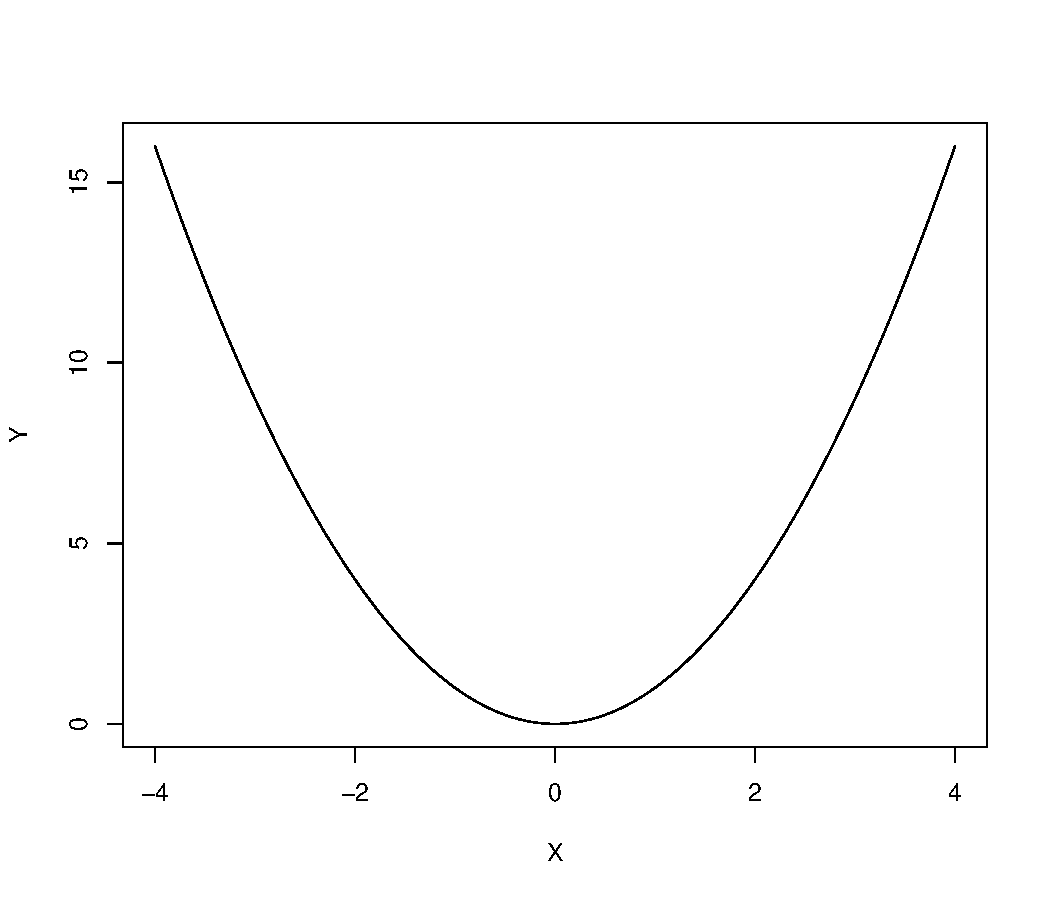
\includegraphics[width=\maxwidth]{figure/unnamed-chunk-2-1} 

}



\end{knitrout}
\end{frame}

\begin{frame}
\frametitle{Pearson correlation coefficient}
$$
\frac{\sum(X - \bar{X})(Y - \bar{Y})}{\sqrt{\sum(X - \bar{X})^2\sum((Y - \bar{Y})^2}}
$$
\end{frame}

\begin{frame}
\frametitle{Calculating Pearson correlation coefficient}
\begin{center}
\begin{tabular}{lll}
\hline
&X	& Y \\
\hline
&5 &	6 \\
&3	&0 \\
&1	&0 \\
\hline
Mean &	3	&2 \\
\hline
\end{tabular}
\end{center}
\begin{knitrout}
\definecolor{shadecolor}{rgb}{0.969, 0.969, 0.969}\color{fgcolor}\begin{kframe}
\begin{alltt}
\hlstd{x} \hlkwb{<-} \hlkwd{c}\hlstd{(}\hlnum{5}\hlstd{,} \hlnum{3}\hlstd{,} \hlnum{1}\hlstd{)}

\hlstd{y} \hlkwb{<-} \hlkwd{c}\hlstd{(}\hlnum{6}\hlstd{,} \hlnum{0}\hlstd{,} \hlnum{0}\hlstd{)}

\hlkwd{cor}\hlstd{(x, y)}
\end{alltt}
\end{kframe}
\end{knitrout}
\end{frame}



\begin{frame}
\frametitle{R correlation applet}
\begin{enumerate}
\item Open RStudio 
\item Open correlation\_applet.R
\item Click the "Source" button
\end{enumerate}
\end{frame}

\begin{frame}
\frametitle{Spearman's rho}
\begin{itemize}
\item Non-parametric measure of association
\item Appropriate when at least one of your variables is ordinal variables
\item Don't use Pearson's correlation with ordinal variables!
\end{itemize}
\end{frame}

\begin{frame}
\frametitle{Simple Linear Regression}
\begin{itemize}
    \item<1-> If are you interested in predicting height given someone's weight, what would you do?
  \item<2-> We could consider a regression model.
  \item<3-> $Y_i = \beta_0 + \beta_1 * X_i$
  \item<4->  \textcolor{red}{How could we assess if this is appropriate?}
\end{itemize}
\end{frame}

\begin{frame}
\frametitle{1993 Growth Survey of 25,000 Hong Kongese children}
\footnotesize \textbf{source:} \url{http://wiki.stat.ucla.edu/socr/index.php/SOCR_Data_Dinov_020108_HeightsWeights}
\begin{knitrout}
\definecolor{shadecolor}{rgb}{0.969, 0.969, 0.969}\color{fgcolor}

{\centering 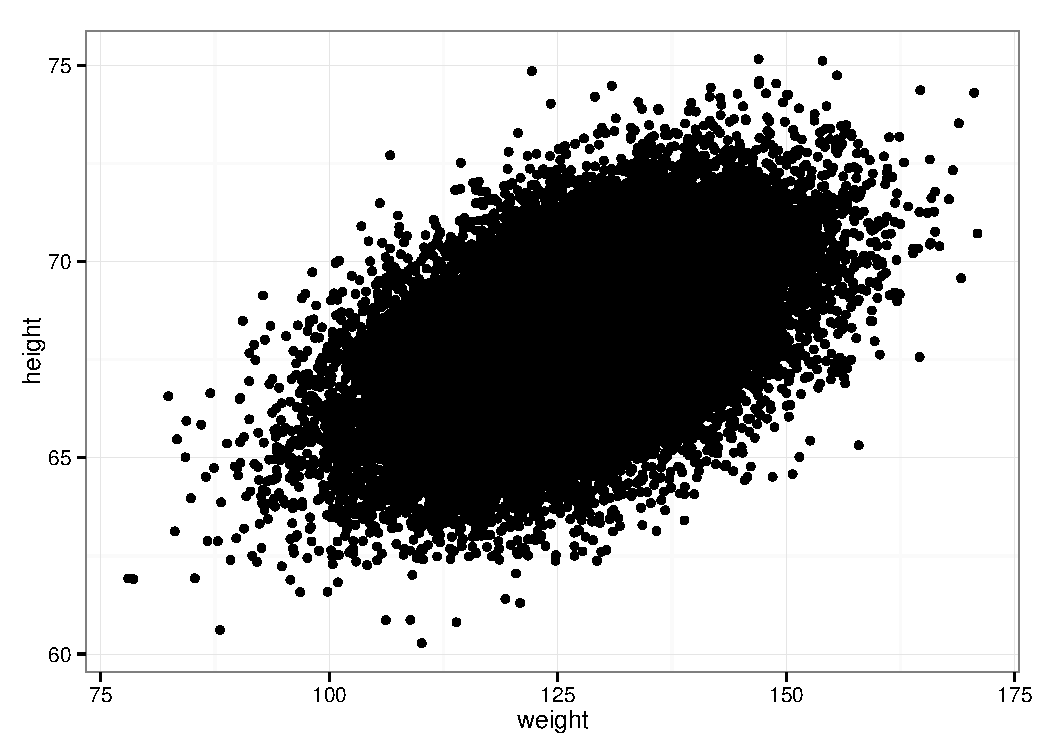
\includegraphics[width=\maxwidth]{figure/unnamed-chunk-4-1} 

}



\end{knitrout}
\end{frame}

\begin{frame}[fragile]
\frametitle{Model Summary}
\begin{tabular}{lllll}
\hline
Parameter & Estimate & SE & t-value & p-value \\
$\beta_0$ & 57.57  & 0.11 & 506.01 & < .001 \\
$\beta_1$ & 0.08 & 0.001 & 91.98 & < .001 \\
\hline
\end{tabular}

\vspace{.5cm}
\textcolor{red}{How does this relate to correlation?}
\end{frame}

\begin{frame}
\frametitle{Slope and the correlation}
\begin{itemize}
\item<1-> There is a relationship between the estimated slope and the correlation between two variables in a simple linear regression.
\item<2-> $r = \beta_1 \frac{sd_x}{sd_y}$ 
\item<3-> If $\beta_1$ = 0.08, the standard deviation of weight and height are 11.6608976 and 1.9016788, respectively, what is r?
\item<4-> 0.5028585
\end{itemize}

\end{frame}

\begin{frame}
\frametitle{Always look at the residuals}
\begin{knitrout}
\definecolor{shadecolor}{rgb}{0.969, 0.969, 0.969}\color{fgcolor}

{\centering 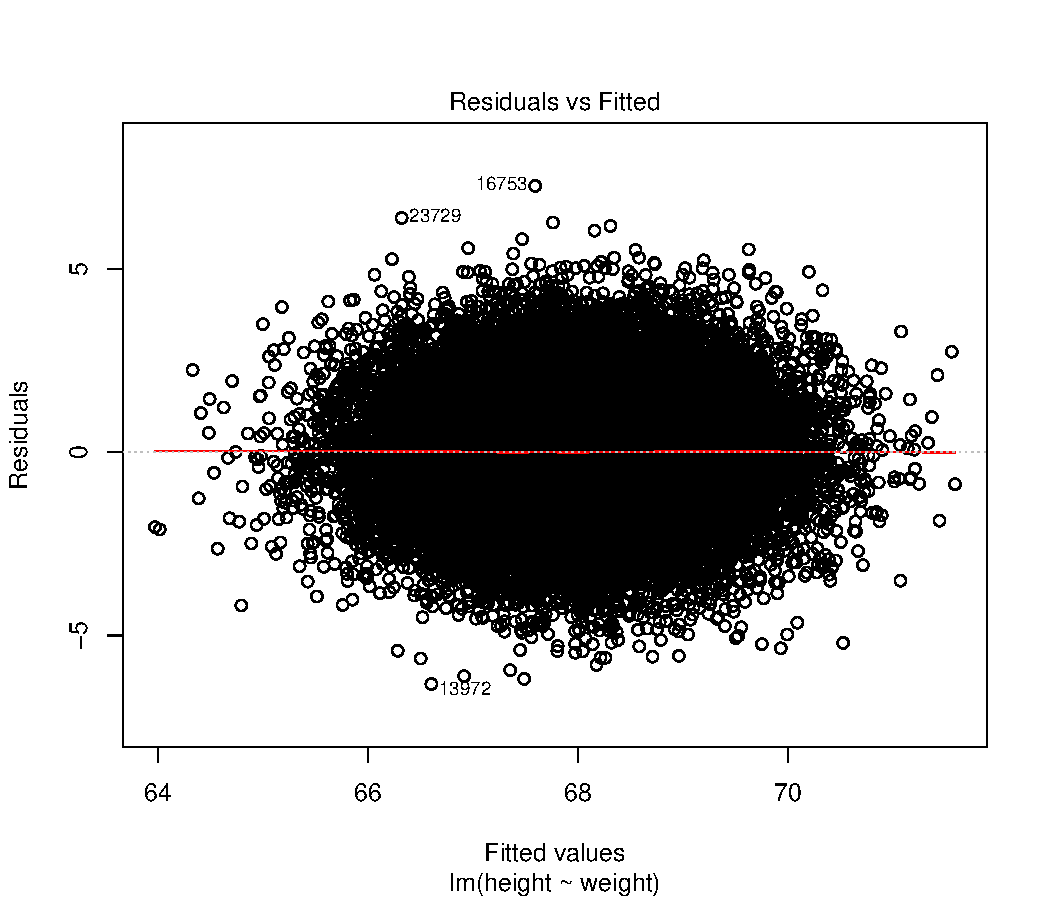
\includegraphics[width=\maxwidth]{figure/unnamed-chunk-5-1} 

}



\end{knitrout}
\end{frame}

\begin{frame}
\frametitle{Brief history of testing}
\begin{itemize}
\item 2200 BCE, Chinese believed to use testing for determining who would get governmental jobs
\item Greek and Romans categorized individuals based on personality type ("blood" or "phlegm")
\item Francis Galton's classification based on "natural gift" (i.e. eugenics)
\begin{itemize}
\item Contributed to development of questionnaries, rating scales, and self-report inventories
\end{itemize}
\item Wilhelm Wundt's laboratory and his focus on "standardization"
\begin{itemize}
\item James Cattell's mental tests
\item Charles Spearman - reliability and factor analysis
\end{itemize}
\end{itemize}
\end{frame}

\begin{frame}
\frametitle{Testing in the 20th century}
\begin{itemize}
\item 1905, Binet and Simon publish a test measuring intelligence in mental retarded school children in Paris
\item 1939, Wechsler publishes a test to measure intelligence in adults (would become WAIS)
\item Group intelligence test administered by the US military during WWI and WWII
\item WWI personality tests used to screen recruits
\end{itemize}
\end{frame}

\begin{frame}
\frametitle{Necessary test assumptions}
\begin{itemize}
\item<1-> Psychological traits and states exist
\item<2-> Psychological traits and states can be measured
\item<3-> Behavior on tests predicts non-test behavior
\item<4-> Measurement error is part of the process
\item<5-> Test can be fair
\item<6-> Test can benefit society
\end{itemize}
\end{frame}

{
\setbeamercolor{normal text}{bg=RoyalBlue}
\begin{frame}
\centering
\Huge \textcolor{white}{What makes a good test?}
\end{frame}
}

\begin{frame}
\frametitle{Norm-Referenced and Standardization}
\begin{itemize}
\item<1-> Individuals scores are relative only to some reference group
\item<2-> This group should represent the entire pool of test takers for the tested construct
\item<3-> Collectively, this group is known as a \textcolor{red}{normative sample} and data from them make up the \textcolor{red}{norms}
\item<4-> Standardization is the process of setting clear procedures for administrating, scoring, and interpreting the test
\item<5-> The normative sample could also be the standardized sample but not always
\item<6-> Understanding the normative sample is very important, why?
\end{itemize}
\end{frame}

\begin{frame}
\frametitle{Sampling}
\begin{itemize}
\item \textcolor{red}{Simple random sample}
\item \textcolor{red}{Stratified random sample}
\item \textcolor{red}{Cluster random sample}
\item Purposive sample
\item Convenience sample
\end{itemize}
\end{frame}

\begin{frame}
\frametitle{Different Norms}
\begin{itemize}
\item Percentiles
\item Developmental Norms
  \begin{itemize}
  \item Age Norms
    \begin{itemize}
    \item A 6 year old performs at the level of a 10 year old
    \item This is on this material only though! 
    \end{itemize}
  \item Grade Norms
    \begin{itemize}
    \item School year typically 10 months in the US
    \item A 4th grader is performing at the level of a 5th grader in third month
    \item This is on this material only though!
    \end{itemize}
  \end{itemize}
\item National Norms, nationally representative
  \begin{itemize}
  \item Anchor norms enable two tests to be compared
  \item In USA, students could take SAT or ACT for admission to college
  \end{itemize}
\end{itemize}
\end{frame}

\begin{frame}
\frametitle{Fixed Reference and Criterion-Related}
\begin{itemize}
\item Fixed reference group scores are used as the basis for calculation of future administrations of the test
\item Raw scores are scaled relative to the performance of the fixed reference group
\begin{itemize}
    \item Answering 50 items correctly one year and 50 on the following year doesn't mean you'll have the same score
  \end{itemize}
\item SAT does this through using anchor items and equating
\item Criterion-referenced, evaluate a score with reference to a set criteria or standard NOT other test takers
\item \textcolor{red}{What is the fairest way to score grades in a class room?}
\end{itemize}
\end{frame}



\end{document}
